\section{Enzymes \& Regulation}

\subsection{Introduction to Enzymes}

\begin{definition}
An \textbf{enzyme} is a biological catalyst, typically a protein, that accelerates the rate of a chemical reaction without being consumed in the process. Enzymes lower the \textbf{activation energy} ($E_a$) required for a reaction to proceed, thereby increasing reaction rates by factors of $10^6$ to $10^{12}$.
\end{definition}

Enzymes are the molecular workhorses of all living cells. Without enzymes, the chemical reactions necessary for life would occur far too slowly to sustain biological processes. Every metabolic pathway, from digestion to DNA replication, depends on specific enzymes working in precise coordination.

The study of enzymes---\textbf{enzymology}---is fundamental to understanding metabolism, drug design, and disease mechanisms. Enzymes exhibit remarkable specificity, typically catalyzing only one reaction or a small set of closely related reactions.

\begin{analogy}
Think of an enzyme like a teacher helping students solve math problems. The students (substrates) could eventually figure out the problem on their own, but it would take a very long time. The teacher (enzyme) helps them understand the problem faster and more efficiently. After helping, the teacher isn't used up---she's ready to help the next group of students!
\end{analogy}

\subsection{Enzyme Nomenclature and Classification}

Enzymes are classified into six major classes based on the type of reaction they catalyze:

\begin{enumerate}[label=\arabic*.]
    \item \textbf{Oxidoreductases:} Catalyze oxidation-reduction (redox) reactions. Transfer electrons between molecules.
    \begin{itemize}
        \item Example: Lactate dehydrogenase (converts lactate to pyruvate)
        \item Common names end in ``-dehydrogenase'' or ``-oxidase''
    \end{itemize}
    
    \item \textbf{Transferases:} Transfer functional groups (amino, phosphate, methyl, etc.) from one molecule to another.
    \begin{itemize}
        \item Example: Hexokinase (transfers phosphate from ATP to glucose)
        \item Common names end in ``-transferase'' or ``-kinase''
    \end{itemize}
    
    \item \textbf{Hydrolases:} Catalyze hydrolysis reactions (breaking bonds using water).
    \begin{itemize}
        \item Example: Trypsin (breaks peptide bonds in proteins)
        \item Common names end in ``-ase'' attached to substrate name
    \end{itemize}
    
    \item \textbf{Lyases:} Add or remove groups to/from double bonds, or form double bonds by removing groups.
    \begin{itemize}
        \item Example: Aldolase (cleaves fructose-1,6-bisphosphate)
        \item Common names include ``-lyase,'' ``-decarboxylase,'' ``-dehydratase''
    \end{itemize}
    
    \item \textbf{Isomerases:} Catalyze structural rearrangements within a single molecule.
    \begin{itemize}
        \item Example: Phosphoglucose isomerase (converts G6P to F6P)
        \item Common names end in ``-isomerase'' or ``-mutase''
    \end{itemize}
    
    \item \textbf{Ligases:} Join two molecules together using ATP energy (forming new bonds).
    \begin{itemize}
        \item Example: DNA ligase (joins DNA fragments)
        \item Common names end in ``-ligase'' or ``-synthetase''
    \end{itemize}
\end{enumerate}

\subsection{Enzyme Structure and the Active Site}

\begin{definition}
The \textbf{active site} is a specific region on an enzyme where substrate binding and catalysis occur. It is typically a three-dimensional cleft or pocket formed by amino acid residues from different parts of the polypeptide chain.
\end{definition}

Key features of the active site:
\begin{enumerate}
    \item \textbf{Specificity:} The shape and chemical properties of the active site determine which substrates can bind
    \item \textbf{Binding residues:} Amino acids that interact with the substrate through hydrogen bonds, ionic interactions, and hydrophobic contacts
    \item \textbf{Catalytic residues:} Amino acids directly involved in the chemical transformation
    \item \textbf{Microenvironment:} The active site often has different properties (pH, polarity) than the surrounding solution
\end{enumerate}

\begin{theorem}
\textbf{Lock-and-Key Model vs. Induced Fit Model:}
\begin{itemize}
    \item \textbf{Lock-and-Key (Emil Fischer, 1894):} The enzyme active site has a rigid, pre-formed shape that exactly matches the substrate, like a key fitting into a lock.
    \item \textbf{Induced Fit (Daniel Koshland, 1958):} The enzyme active site is flexible and changes shape upon substrate binding to achieve optimal fit. This is the more accurate modern understanding.
\end{itemize}
\end{theorem}

\begin{analogy}
The lock-and-key model is like putting your hand into a rigid glove that's exactly your size. The induced fit model is like putting your hand into a flexible mitten---the mitten adjusts and wraps around your hand to create a snug fit. Most enzymes work more like the mitten!
\end{analogy}

\subsection{Cofactors and Coenzymes}

Many enzymes require non-protein molecules called \textbf{cofactors} for activity.

\begin{definition}
\begin{itemize}
    \item \textbf{Cofactor:} A non-protein molecule required for enzyme activity. Can be inorganic (metal ions) or organic (coenzymes).
    \item \textbf{Coenzyme:} An organic cofactor, often derived from vitamins, that participates in the catalytic reaction.
    \item \textbf{Prosthetic group:} A cofactor that is tightly or covalently bound to the enzyme.
    \item \textbf{Apoenzyme:} The protein portion of an enzyme without its cofactor.
    \item \textbf{Holoenzyme:} The complete, catalytically active enzyme (apoenzyme + cofactor).
\end{itemize}
\end{definition}

\begin{center}
\begin{tabular}{lll}
\toprule
\textbf{Cofactor Type} & \textbf{Examples} & \textbf{Function} \\
\midrule
Metal ions & Zn$^{2+}$, Mg$^{2+}$, Fe$^{2+}$, Cu$^{2+}$ & Stabilize charges, participate in redox \\
NAD$^+$/NADH & From niacin (B3) & Electron carrier in redox reactions \\
FAD/FADH$_2$ & From riboflavin (B2) & Electron carrier in redox reactions \\
Coenzyme A & From pantothenic acid (B5) & Acyl group carrier \\
Thiamine pyrophosphate & From thiamine (B1) & Decarboxylation reactions \\
Pyridoxal phosphate & From pyridoxine (B6) & Amino acid metabolism \\
Biotin & Vitamin B7 & Carboxylation reactions \\
Tetrahydrofolate & From folic acid & One-carbon transfers \\
\bottomrule
\end{tabular}
\end{center}

\subsection{Mechanisms of Enzyme Catalysis}

Enzymes accelerate reactions through several mechanisms:

\begin{enumerate}[label=\arabic*.]
    \item \textbf{Proximity and Orientation Effects:} Enzymes bring substrates together in the correct orientation for reaction, increasing the effective concentration of reactants.
    
    \item \textbf{Transition State Stabilization:} Enzymes preferentially bind and stabilize the transition state, lowering the activation energy. This is the most important catalytic mechanism.
    
    \item \textbf{Acid-Base Catalysis:} Amino acid residues donate or accept protons during the reaction.
    \begin{itemize}
        \item General acid catalysis: Proton donation
        \item General base catalysis: Proton acceptance
    \end{itemize}
    
    \item \textbf{Covalent Catalysis:} A covalent bond forms transiently between the enzyme and substrate.
    \begin{itemize}
        \item Example: Serine proteases form acyl-enzyme intermediates
    \end{itemize}
    
    \item \textbf{Metal Ion Catalysis:} Metal ions stabilize negative charges, participate in redox reactions, or activate water molecules.
\end{enumerate}

\begin{example}
\textbf{Chymotrypsin Mechanism:}

Chymotrypsin is a serine protease that cleaves peptide bonds. It uses a \textbf{catalytic triad} consisting of Ser195, His57, and Asp102.

\textbf{Step 1:} His57 acts as a general base, abstracting a proton from Ser195, making it a powerful nucleophile.

\textbf{Step 2:} The activated Ser195 attacks the carbonyl carbon of the peptide bond (covalent catalysis), forming a tetrahedral intermediate.

\textbf{Step 3:} The tetrahedral intermediate collapses, releasing the first product (amine portion) and forming an acyl-enzyme intermediate.

\textbf{Step 4:} Water attacks the acyl-enzyme intermediate, forming another tetrahedral intermediate.

\textbf{Step 5:} The second tetrahedral intermediate collapses, releasing the carboxylic acid product and regenerating free enzyme.
\end{example}

\subsection{Enzyme Regulation}

Cells must precisely control enzyme activity to maintain homeostasis and respond to changing conditions. Several regulatory mechanisms exist:

\subsubsection{Allosteric Regulation}

\begin{definition}
\textbf{Allosteric regulation} occurs when a molecule binds to a site on the enzyme \textit{other than} the active site (the allosteric site), causing a conformational change that affects enzyme activity.
\end{definition}

\begin{itemize}
    \item \textbf{Allosteric activators:} Increase enzyme activity by stabilizing the active (R) state
    \item \textbf{Allosteric inhibitors:} Decrease enzyme activity by stabilizing the inactive (T) state
    \item \textbf{Homotropic effectors:} The substrate itself acts as an allosteric modulator
    \item \textbf{Heterotropic effectors:} A molecule other than the substrate acts as the modulator
\end{itemize}

\begin{analogy}
Imagine a door with two handles---one on the front (active site) and one on the back (allosteric site). Normally, you open the door by turning the front handle. But if someone holds the back handle in a certain way, it can either make the front handle easier to turn (activator) or lock it so it won't turn at all (inhibitor). The person at the back controls how well the front handle works!
\end{analogy}

\begin{theorem}
\textbf{Concerted (MWC) Model of Allostery:}
\begin{itemize}
    \item Enzyme exists in equilibrium between T (tense, low affinity) and R (relaxed, high affinity) states
    \item All subunits change conformation simultaneously (concerted)
    \item Substrates preferentially bind R state, shifting equilibrium toward R
    \item Inhibitors stabilize T state; activators stabilize R state
\end{itemize}
\end{theorem}

\subsubsection{Covalent Modification}

\begin{definition}
\textbf{Covalent modification} involves the addition or removal of chemical groups to/from the enzyme, altering its activity. The most common modification is \textbf{phosphorylation}.
\end{definition}

\begin{itemize}
    \item \textbf{Phosphorylation:} Addition of phosphate group by kinases; removal by phosphatases
    \begin{itemize}
        \item Adds negative charges, can activate or inhibit depending on enzyme
        \item Example: Glycogen phosphorylase is activated by phosphorylation
        \item Example: Glycogen synthase is inhibited by phosphorylation
    \end{itemize}
    \item \textbf{Acetylation:} Addition of acetyl groups
    \item \textbf{Methylation:} Addition of methyl groups
    \item \textbf{Ubiquitination:} Addition of ubiquitin proteins (often targets for degradation)
\end{itemize}

\subsubsection{Proteolytic Activation (Zymogens)}

\begin{definition}
A \textbf{zymogen} (or proenzyme) is an inactive enzyme precursor that requires proteolytic cleavage to become active. This is an irreversible activation mechanism.
\end{definition}

\begin{example}
\textbf{Digestive Enzyme Zymogens:}
\begin{itemize}
    \item Pepsinogen $\xrightarrow{\text{HCl, pepsin}}$ Pepsin (in stomach)
    \item Trypsinogen $\xrightarrow{\text{enteropeptidase}}$ Trypsin (in small intestine)
    \item Chymotrypsinogen $\xrightarrow{\text{trypsin}}$ Chymotrypsin
\end{itemize}

\textbf{Why zymogens?} They prevent enz
ymes from digesting the cells that produce them. Pancreatic cells would be destroyed if trypsin were active inside them!
\end{example}

\subsubsection{Isozymes}

\begin{definition}
\textbf{Isozymes} (or isoenzymes) are different molecular forms of the same enzyme that catalyze the same reaction but differ in kinetic properties, regulatory properties, or tissue distribution.
\end{definition}

\begin{example}
\textbf{Lactate Dehydrogenase (LDH) Isozymes:}

LDH is a tetramer composed of H (heart) and M (muscle) subunits:
\begin{itemize}
    \item LDH-1 (H4): Predominant in heart, high affinity for lactate
    \item LDH-2 (H3M1): Found in RBCs
    \item LDH-3 (H2M2): Found in brain, kidney
    \item LDH-4 (HM3): Found in kidney, placenta
    \item LDH-5 (M4): Predominant in liver and skeletal muscle, high affinity for pyruvate
\end{itemize}

\textbf{Clinical Application:} Elevated LDH-1 in blood indicates heart damage (myocardial infarction). Different isozyme patterns help diagnose tissue-specific damage.
\end{example}

\subsection{Feedback Inhibition in Metabolic Pathways}

\begin{definition}
\textbf{Feedback inhibition} occurs when the end product of a metabolic pathway inhibits an enzyme early in the pathway, preventing overproduction of the product.
\end{definition}

\begin{analogy}
Feedback inhibition is like a thermostat. When your house gets warm enough, the thermostat tells the heater to turn off. The "product" (warm air) inhibits the "enzyme" (heater) to prevent overheating. Similarly, when a cell has enough of a product, that product tells the pathway to slow down.
\end{analogy}

\begin{example}
\textbf{Isoleucine Biosynthesis:}

\begin{center}
Threonine $\xrightarrow{\text{threonine deaminase}}$ $\alpha$-ketobutyrate $\rightarrow$ ... $\rightarrow$ Isoleucine
\end{center}

When isoleucine accumulates, it allosterically inhibits threonine deaminase (the first committed step), preventing unnecessary synthesis.
\end{example}

\subsection{Regulation Summary Table}

\begin{center}
\begin{tabular}{|l|l|l|l|}
\hline
\textbf{Mechanism} & \textbf{Speed} & \textbf{Reversibility} & \textbf{Example} \\
\hline
Allosteric regulation & Fast (seconds) & Reversible & PFK-1, ATCase \\
\hline
Covalent modification & Moderate (minutes) & Reversible & Glycogen phosphorylase \\
\hline
Proteolytic cleavage & Slow (minutes-hours) & Irreversible & Trypsinogen $\rightarrow$ trypsin \\
\hline
Gene expression & Slow (hours-days) & Reversible & Enzyme induction \\
\hline
\end{tabular}
\end{center}

%================================================================
% SECTION 8: ENZYME KINETICS
%================================================================

\section{Enzyme Kinetics}

\subsection{Introduction to Enzyme Kinetics}

\begin{definition}
\textbf{Enzyme kinetics} is the study of the rates of enzyme-catalyzed reactions and how these rates are affected by various factors including substrate concentration, enzyme concentration, pH, temperature, and the presence of inhibitors or activators.
\end{definition}

\begin{analogy}
Think of enzyme kinetics like studying how fast a pizza restaurant can make pizzas. The "rate" is how many pizzas per hour. This depends on how many orders come in (substrate concentration), how many chefs are working (enzyme concentration), whether the ovens are at the right temperature, and whether anything is slowing down the kitchen (inhibitors).
\end{analogy}

\subsection{Reaction Velocity and Substrate Concentration}

\subsubsection{The Michaelis-Menten Model}

\begin{definition}
The \textbf{Michaelis-Menten model} describes the kinetics of many enzymes by relating reaction velocity ($v$) to substrate concentration ([S]).
\end{definition}

\begin{theorem}
\textbf{Michaelis-Menten Equation:}
\[
v = \frac{V_{\max}[S]}{K_m + [S]}
\]

Where:
\begin{itemize}
    \item $v$ = initial reaction velocity
    \item $V_{\max}$ = maximum velocity (when enzyme is saturated)
    \item $[S]$ = substrate concentration
    \item $K_m$ = Michaelis constant (substrate concentration at $\frac{1}{2}V_{\max}$)
\end{itemize}
\end{theorem}

\subsubsection{Derivation of the Michaelis-Menten Equation}

The model assumes a simple reaction mechanism:

\[
E + S \underset{k_{-1}}{\stackrel{k_1}{\rightleftharpoons}} ES \xrightarrow{k_2} E + P
\]

\textbf{Key Assumptions:}
\begin{enumerate}
    \item \textbf{Steady-state assumption:} The concentration of ES remains constant over time (rate of ES formation = rate of ES breakdown)
    \item \textbf{Initial velocity conditions:} Measured before significant product accumulates (so reverse reaction $P \rightarrow S$ is negligible)
    \item $[S] >> [E]_{\text{total}}$, so substrate concentration doesn't change significantly
\end{enumerate}

\textbf{Derivation Steps:}

1. Rate of ES formation: $k_1[E][S]$

2. Rate of ES breakdown: $k_{-1}[ES] + k_2[ES] = (k_{-1} + k_2)[ES]$

3. At steady state: $k_1[E][S] = (k_{-1} + k_2)[ES]$

4. Define $K_m = \frac{k_{-1} + k_2}{k_1}$ (Michaelis constant)

5. Total enzyme: $[E]_{\text{total}} = [E] + [ES]$, so $[E] = [E]_{\text{total}} - [ES]$

6. Substituting and solving for [ES]:
\[
[ES] = \frac{[E]_{\text{total}}[S]}{K_m + [S]}
\]

7. Reaction velocity: $v = k_2[ES] = \frac{k_2[E]_{\text{total}}[S]}{K_m + [S]}$

8. Since $V_{\max} = k_2[E]_{\text{total}}$:
\[
\boxed{v = \frac{V_{\max}[S]}{K_m + [S]}}
\]

\subsection{Understanding Kinetic Parameters}

\subsubsection{$V_{\max}$ (Maximum Velocity)}

\begin{definition}
$V_{\max}$ is the maximum rate of the reaction when the enzyme is fully saturated with substrate (all enzyme molecules are in the ES complex).
\end{definition}

\begin{itemize}
    \item $V_{\max} = k_2[E]_{\text{total}} = k_{\text{cat}}[E]_{\text{total}}$
    \item Directly proportional to enzyme concentration
    \item Units: M/s, $\mu$mol/min, etc.
    \item Increasing [E] increases $V_{\max}$
\end{itemize}

\subsubsection{$K_m$ (Michaelis Constant)}

\begin{definition}
$K_m$ is the substrate concentration at which the reaction velocity is half of $V_{\max}$. It is a measure of the enzyme's affinity for its substrate.
\end{definition}

\begin{itemize}
    \item \textbf{Low $K_m$:} High affinity (enzyme reaches half-maximal velocity at low [S])
    \item \textbf{High $K_m$:} Low affinity (enzyme needs high [S] to reach half-maximal velocity)
    \item Units: Concentration (M, mM, $\mu$M)
    \item $K_m$ is independent of enzyme concentration
    \item $K_m$ is characteristic of each enzyme-substrate pair
\end{itemize}

\begin{analogy}
$K_m$ is like how hungry you are for pizza. If you have a low $K_m$ for pizza, even the smell of one slice (low concentration) gets you halfway to full satisfaction. If you have a high $K_m$, you need a whole pizza shop's worth before you're even halfway interested. Low $K_m$ = high affinity = easily satisfied!
\end{analogy}

\subsubsection{$k_{\text{cat}}$ (Turnover Number)}

\begin{definition}
The \textbf{turnover number} ($k_{\text{cat}}$) is the number of substrate molecules converted to product per enzyme molecule per unit time when the enzyme is saturated.
\end{definition}

\[
k_{\text{cat}} = \frac{V_{\max}}{[E]_{\text{total}}}
\]

\begin{itemize}
    \item Units: s$^{-1}$ (per second)
    \item Represents the intrinsic catalytic efficiency of the enzyme
    \item Also called the "molecular activity"
\end{itemize}

\begin{example}
\textbf{Turnover Numbers of Various Enzymes:}
\begin{center}
\begin{tabular}{|l|c|}
\hline
\textbf{Enzyme} & \textbf{$k_{\text{cat}}$ (s$^{-1}$)} \\
\hline
Carbonic anhydrase & $6 \times 10^5$ \\
\hline
Catalase & $4 \times 10^7$ \\
\hline
Chymotrypsin & 100 \\
\hline
Lysozyme & 0.5 \\
\hline
\end{tabular}
\end{center}

Carbonic anhydrase converts 600,000 CO$_2$ molecules to bicarbonate per second!
\end{example}

\subsubsection{Catalytic Efficiency ($k_{\text{cat}}/K_m$)}

\begin{definition}
\textbf{Catalytic efficiency} ($k_{\text{cat}}/K_m$) measures how efficiently an enzyme converts substrate to product when substrate is limiting. It accounts for both binding affinity and catalytic speed.
\end{definition}

\begin{itemize}
    \item Units: M$^{-1}$s$^{-1}$
    \item Upper limit is the diffusion-controlled limit: $\sim 10^8 - 10^9$ M$^{-1}$s$^{-1}$
    \item Enzymes approaching this limit are called \textbf{catalytically perfect}
    \item Useful for comparing different enzymes or same enzyme with different substrates
\end{itemize}

\begin{example}
\textbf{Catalytically Perfect Enzymes:}

Triose phosphate isomerase has $k_{\text{cat}}/K_m \approx 2 \times 10^8$ M$^{-1}$s$^{-1}$, approaching the diffusion limit. Every collision between enzyme and substrate results in product formation!
\end{example}

\subsection{Graphical Analysis of Enzyme Kinetics}

\subsubsection{Michaelis-Menten Plot}

\begin{center}
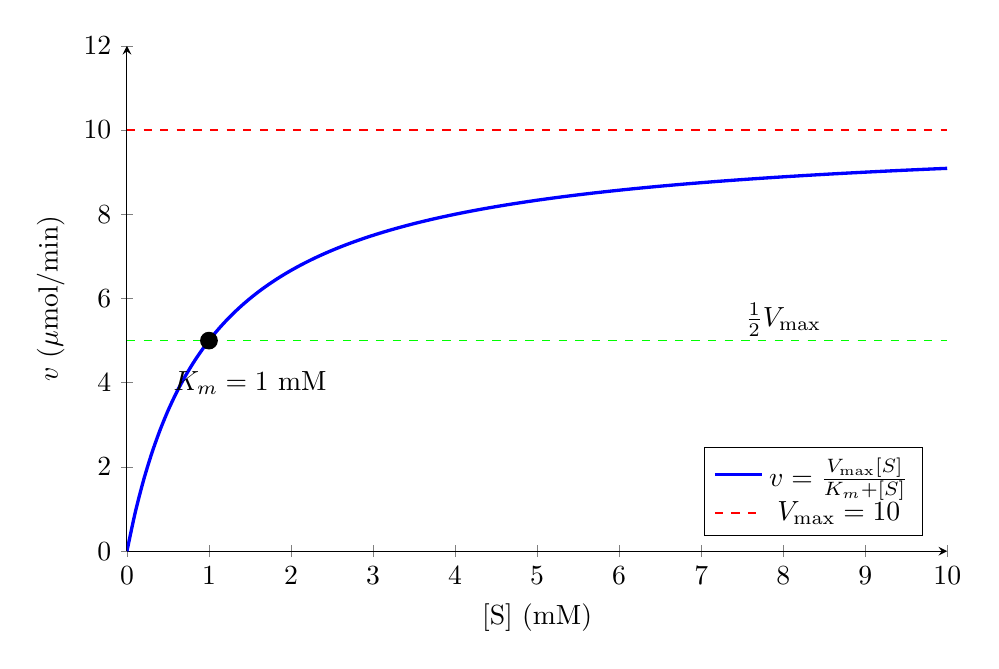
\begin{tikzpicture}
\begin{axis}[
    xlabel={[S] (mM)},
    ylabel={$v$ ($\mu$mol/min)},
    xmin=0, xmax=10,
    ymin=0, ymax=12,
    axis lines=left,
    width=12cm,
    height=8cm,
    legend pos=south east
]
% Michaelis-Menten curve
\addplot[blue, very thick, smooth, domain=0:10, samples=100] {10*x/(1+x)};
\addlegendentry{$v = \frac{V_{\max}[S]}{K_m + [S]}$}

% Vmax line
\addplot[red, dashed, thick, domain=0:10] {10};
\addlegendentry{$V_{\max} = 10$}

% Half Vmax line
\addplot[green, dashed, domain=0:10] {5};

% Km marker
\addplot[only marks, mark=*, mark size=3pt] coordinates {(1,5)};
\node at (axis cs:1.5,4) {$K_m = 1$ mM};
\node at (axis cs:8,5.5) {$\frac{1}{2}V_{\max}$};

\end{axis}
\end{tikzpicture}
\end{center}

\textbf{Key Features:}
\begin{itemize}
    \item Hyperbolic curve approaching $V_{\max}$ asymptotically
    \item At low [S]: $v \approx \frac{V_{\max}}{K_m}[S]$ (first-order kinetics)
    \item At high [S]: $v \approx V_{\max}$ (zero-order kinetics)
    \item At [S] = $K_m$: $v = \frac{1}{2}V_{\max}$
\end{itemize}

\subsubsection{Lineweaver-Burk Plot (Double Reciprocal Plot)}

Taking the reciprocal of the Michaelis-Menten equation:

\begin{theorem}
\textbf{Lineweaver-Burk Equation:}
\[
\frac{1}{v} = \frac{K_m}{V_{\max}} \cdot \frac{1}{[S]} + \frac{1}{V_{\max}}
\]

This is in the form $y = mx + b$, giving a straight line when $\frac{1}{v}$ is plotted against $\frac{1}{[S]}$.
\end{theorem}

\begin{center}
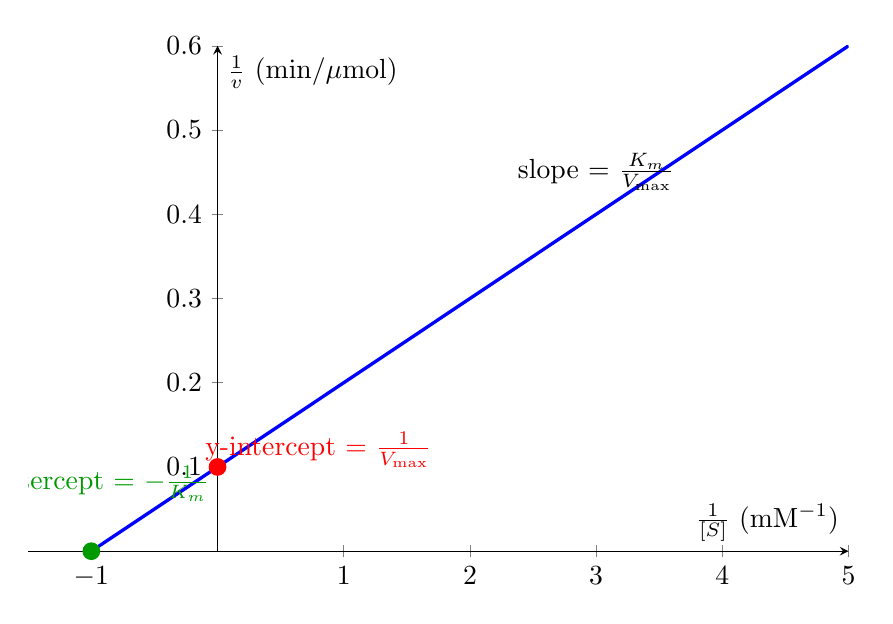
\begin{tikzpicture}
\begin{axis}[
    xlabel={$\frac{1}{[S]}$ (mM$^{-1}$)},
    ylabel={$\frac{1}{v}$ (min/$\mu$mol)},
    xmin=-1.5, xmax=5,
    ymin=0, ymax=0.6,
    axis lines=center,
    width=12cm,
    height=8cm,
]
% Lineweaver-Burk line
\addplot[blue, very thick, domain=-1:5] {0.1 + 0.1*x};

% Intercept markers
\addplot[only marks, mark=*, mark size=3pt, red] coordinates {(0,0.1)};
\node[red] at (axis cs:0.8,0.12) {y-intercept = $\frac{1}{V_{\max}}$};

\addplot[only marks, mark=*, mark size=3pt, green!60!black] coordinates {(-1,0)};
\node[green!60!black] at (axis cs:-1,0.08) {x-intercept = $-\frac{1}{K_m}$};

% Slope annotation
\node at (axis cs:3,0.45) {slope = $\frac{K_m}{V_{\max}}$};

\end{axis}
\end{tikzpicture}
\end{center}

\textbf{Key Features:}
\begin{itemize}
    \item y-intercept = $\frac{1}{V_{\max}}$
    \item x-intercept = $-\frac{1}{K_m}$
    \item Slope = $\frac{K_m}{V_{\max}}$
    \item Useful for determining kinetic parameters and analyzing inhibition
\end{itemize}

\subsection{Enzyme Inhibition}

\begin{definition}
\textbf{Enzyme inhibition} is the decrease in enzyme activity caused by the binding of specific molecules (inhibitors) to the enzyme.
\end{definition}

\subsubsection{Reversible Inhibition}

\textbf{1. Competitive Inhibition}

\begin{definition}
A \textbf{competitive inhibitor} binds to the active site of the enzyme, competing directly with the substrate for binding.
\end{definition}

\begin{itemize}
    \item Inhibitor resembles substrate structurally
    \item Effect can be overcome by increasing [S]
    \item $K_m$ increases (apparent lower affinity)
    \item $V_{\max}$ unchanged (at infinite [S], all inhibitor is displaced)
\end{itemize}

\[
v = \frac{V_{\max}[S]}{K_m\left(1 + \frac{[I]}{K_i}\right) + [S]} = \frac{V_{\max}[S]}{K_m^{\text{app}} + [S]}
\]

where $K_m^{\text{app}} = K_m\left(1 + \frac{[I]}{K_i}\right)$

\begin{example}
\textbf{Methotrexate} is a competitive inhibitor of dihydrofolate reductase (DHFR). It resembles the substrate dihydrofolate and is used as a chemotherapy drug because rapidly dividing cancer cells require folate for DNA synthesis.
\end{example}

\textbf{2. Uncompetitive Inhibition}

\begin{definition}
An \textbf{uncompetitive inhibitor} binds only to the enzyme-substrate (ES) complex, not to the free enzyme.
\end{definition}

\begin{itemize}
    \item Inhibitor binds to a site created when substrate binds
    \item Both $K_m$ and $V_{\max}$ decrease by the same factor
    \item Cannot be overcome by increasing [S]
    \item Lineweaver-Burk: parallel lines (same slope)
\end{itemize}

\[
v = \frac{V_{\max}^{\text{app}}[S]}{K_m^{\text{app}} + [S]}
\]

where $V_{\max}^{\text{app}} = \frac{V_{\max}}{1 + \frac{[I]}{K_i}}$ and $K_m^{\text{app}} = \frac{K_m}{1 + \frac{[I]}{K_i}}$

\textbf{3. Noncompetitive Inhibition (Mixed Inhibition)}

\begin{definition}
A \textbf{noncompetitive inhibitor} binds to a site other than the active site and can bind to either the free enzyme (E) or the enzyme-substrate complex (ES).
\end{definition}

\begin{itemize}
    \item Pure noncompetitive: binds E and ES with equal affinity
    \item $V_{\max}$ decreases (fewer functional enzyme molecules)
    \item $K_m$ unchanged (in pure noncompetitive)
    \item Cannot be overcome by increasing [S]
\end{itemize}

\[
v = \frac{V_{\max}^{\text{app}}[S]}{K_m + [S]}
\]

where $V_{\max}^{\text{app}} = \frac{V_{\max}}{1 + \frac{[I]}{K_i}}$

\begin{analogy}
\textbf{Types of Inhibition - A Restaurant Analogy:}
\begin{itemize}
    \item \textbf{Competitive:} Another customer sits in your reserved seat. If you wait long enough (more customers = more substrate), you'll eventually get a seat.
    \item \textbf{Uncompetitive:} A health inspector closes tables only after customers sit down. Fewer tables available, but also fewer customers can even try to sit.
    \item \textbf{Noncompetitive:} The chef gets sick. It doesn't matter how many customers come—the kitchen can only work at half capacity.
\end{itemize}
\end{analogy}

\subsubsection{Summary of Reversible Inhibition}

\begin{center}
\begin{tabular}{lccc}
\toprule
\textbf{Inhibition Type} & \textbf{Binds To} & \textbf{$K_m$} & \textbf{$V_{\max}$} \\
\midrule
Competitive & E only & Increases & Unchanged \\
Uncompetitive & ES only & Decreases & Decreases \\
Noncompetitive (pure) & E and ES & Unchanged & Decreases \\
\bottomrule
\end{tabular}
\end{center}

\begin{center}
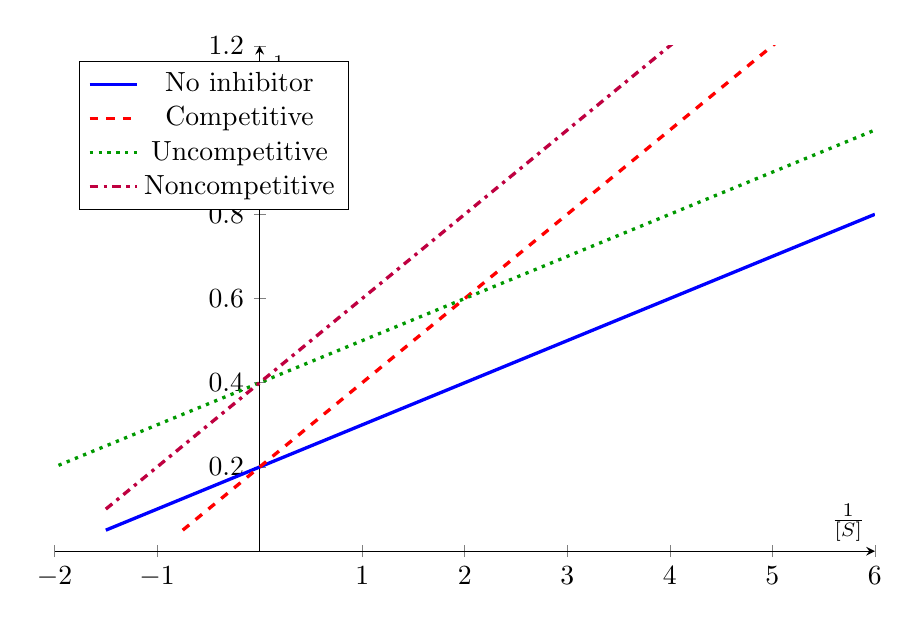
\begin{tikzpicture}
\begin{axis}[
    xlabel={$\frac{1}{[S]}$},
    ylabel={$\frac{1}{v}$},
    xmin=-2, xmax=6,
    ymin=0, ymax=1.2,
    axis lines=center,
    width=12cm,
    height=8cm,
    legend pos=north west,
]
% No inhibitor
\addplot[blue, very thick, domain=-1.5:6] {0.2 + 0.1*x};
\addlegendentry{No inhibitor}

% Competitive
\addplot[red, very thick, dashed, domain=-0.75:6] {0.2 + 0.2*x};
\addlegendentry{Competitive}

% Uncompetitive
\addplot[green!60!black, very thick, dotted, domain=-3:6] {0.4 + 0.1*x};
\addlegendentry{Uncompetitive}

% Noncompetitive
\addplot[purple, very thick, dashdotted, domain=-1.5:6] {0.4 + 0.2*x};
\addlegendentry{Noncompetitive}

\end{axis}
\end{tikzpicture}
\end{center}

\subsubsection{Irreversible Inhibition}

\begin{definition}
\textbf{Irreversible inhibitors} form covalent bonds with the enzyme, permanently inactivating it. The enzyme must be replaced by new protein synthesis.
\end{definition}

\begin{example}
\textbf{Examples of Irreversible Inhibitors:}
\begin{itemize}
    \item \textbf{Aspirin:} Acetylates cyclooxygenase (COX), blocking prostaglandin synthesis
    \item \textbf{Penicillin:} Covalently modifies transpeptidase, preventing bacterial cell wall synthesis
    \item \textbf{Organophosphates} (nerve agents, pesticides): Phosphorylate acetylcholinesterase
    \item \textbf{DIPF} (diisopropyl fluorophosphate): Modifies serine in serine proteases
\end{itemize}
\end{example}

\subsection{Catalytic Efficiency}

\begin{definition}
The \textbf{catalytic efficiency} of an enzyme is measured by the ratio $\frac{k_{\text{cat}}}{K_m}$, which accounts for both the rate of catalysis and substrate binding.
\end{definition}

\begin{itemize}
    \item $k_{\text{cat}}$ (turnover number) = $\frac{V_{\max}}{[E]_T}$ = molecules of substrate converted per enzyme per unit time
    \item Units of $k_{\text{cat}}$: s$^{-1}$
    \item Units of $\frac{k_{\text{cat}}}{K_m}$: M$^{-1}$s$^{-1}$
    \item Maximum theoretical limit: $10^8 - 10^9$ M$^{-1}$s$^{-1}$ (diffusion-controlled)
\end{itemize}

\begin{example}
\textbf{Catalase} has one of the highest $k_{\text{cat}}$ values known:
\begin{itemize}
    \item $k_{\text{cat}} \approx 4 \times 10^7$ s$^{-1}$
    \item This means each catalase molecule converts 40 million H$_2$O$_2$ molecules to H$_2$O and O$_2$ every second!
\end{itemize}
\end{example}

\begin{theorem}
\textbf{Specificity Constant:}

The ratio $\frac{k_{\text{cat}}}{K_m}$ is called the specificity constant and is used to compare:
\begin{itemize}
    \item The efficiency of different enzymes
    \item The preference of one enzyme for different substrates
    \item Higher $\frac{k_{\text{cat}}}{K_m}$ = better enzyme or preferred substrate
\end{itemize}
\end{theorem}

\subsection{Enzyme Kinetics Problem-Solving Strategies}

\begin{skillbox}
\textbf{Calculating $K_m$ and $V_{\max}$ from Data:}

\textbf{Method 1: Direct Inspection}
\begin{enumerate}
    \item Find $V_{\max}$ as the plateau value at high [S]
    \item Find $\frac{V_{\max}}{2}$
    \item $K_m$ = [S] at which $v = \frac{V_{\max}}{2}$
\end{enumerate}

\textbf{Method 2: Lineweaver-Burk Plot}
\begin{enumerate}
    \item Calculate $\frac{1}{v}$ and $\frac{1}{[S]}$ for each data point
    \item Plot $\frac{1}{v}$ vs $\frac{1}{[S]}$
    \item y-intercept = $\frac{1}{V_{\max}}$
    \item x-intercept = $-\frac{1}{K_m}$
\end{enumerate}
\end{skillbox}

\begin{example}
Given the following kinetic data, determine $K_m$ and $V_{\max}$:

\begin{center}
\begin{tabular}{cc}
\toprule
{[S] (mM)} & $v$ ($\mu$mol/min) \\
\midrule
0.5 & 25 \\
1.0 & 40 \\
2.0 & 57 \\
4.0 & 73 \\
8.0 & 84 \\
16.0 & 92 \\
\bottomrule
\end{tabular}
\end{center}
\end{example}

\begin{solution}
\textbf{Using Lineweaver-Burk Plot:}

First, calculate reciprocals:
\begin{center}
\begin{tabular}{cccc}
\toprule
{[S] (mM)} & $v$ ($\mu$mol/min) & $\frac{1}{[S]}$ (mM$^{-1}$) & $\frac{1}{v}$ (min/$\mu$mol) \\
\midrule
0.5 & 25 & 2.0 & 0.040 \\
1.0 & 40 & 1.0 & 0.025 \\
2.0 & 57 & 0.5 & 0.018 \\
4.0 & 73 & 0.25 & 0.014 \\
8.0 & 84 & 0.125 & 0.012 \\
16.0 & 92 & 0.0625 & 0.011 \\
\bottomrule
\end{tabular}
\end{center}

From linear regression or graphical analysis:
\begin{itemize}
    \item y-intercept $\approx 0.010$ min/$\mu$mol
    \item Therefore: $V_{\max} = \frac{1}{0.010} = 100$ $\mu$mol/min
    \item x-intercept $\approx -1.0$ mM$^{-1}$
    \item Therefore: $K_m = -\frac{1}{-1.0} = 1.0$ mM
\end{itemize}

\textbf{Verification:} At [S] = $K_m$ = 1.0 mM, $v$ should equal $\frac{V_{\max}}{2} = 50$ $\mu$mol/min.

The measured value is 40 $\mu$mol/min, which is close (experimental error accounts for difference).
\end{solution}

%================================================================
% SECTION 9: BIOCHEMICAL ENERGY, METABOLISM, CARBOHYDRATES
%================================================================

